\documentclass[a4paper,english]{article}
\usepackage{graphicx}
\usepackage{listings}
\usepackage{amsmath}
\usepackage{multirow}
%% Use utf-8 encoding for foreign characters
%%\usepackage[T1]{fontenc}
%%\usepackage[utf8]{inputenc}
%%\usepackage{babel}
%%
%%%% Vector based fonts instead of bitmaps
%%\usepackage{lmodern}
%%
%%%% Useful
%%%\usepackage{fullpage} % Smaller margins
%%\usepackage{enumerate}
%%
%%%% Theorem
%%\usepackage{amsthm}
%%
%%%% More math
%%\usepackage{amsmath}
%%\usepackage{amssymb}
\lstset{
  breaklines=true,
  postbreak=\mbox{{$\hookrightarrow$}\space},
  numbers=left,
}
%% Document Header
\title{Section5}
\author{Elliott Ashby}
\date{\today}

\begin{document}
    \maketitle
    \section{Write a program to model the one-dimensional Uranium.}
    \lstinputlisting[language=Python, firstline=7, lastline=37]{./4.py}
    This code has 2 functions, neutron which returns a location between 0 and L and the number of nuetrons from the fission
    (in this case 2). And the other function is chain, which takes a location, number of neutrons and L. It then randomly 
    determines which direction the neutrons travel and excludes them if they are outside the range of 0 to L. It then
    returns the number of total nuetrons that stay within the range.
    \\
    \section{Create an updated version of your program using the neutrons() function.}
    \lstinputlisting[language=Python, firstline=40, lastline=44]{./4.py}
    Here, we simply change the number of neutrons to be set by the neutrons.neutrons() function and not a static 2.
    \section{Start with L = 0.1m and vary this to determine the critical value. Decide
whether you need to use more than 100 initial neutrons}
    \lstinputlisting[language=Python, firstline=65, lastline=77]{./4.py}
    Here we update neutron to include the function neutrons which returns a random number with average of 2.5 and make 
    a new while loop in order to determine the critical value. It does this by taking an average count of secondary fissions
    of 1000 fissions each with 100 initial fissions. Once the average is larger than the inital fissions, it means more 
    secondary fissions occur than initial fissions.
    Using this we get a critical value:
    \begin{center}
        $L_{critical value} \approx 0.142 \pm 0.0005$
    \end{center}
    Using more than 100 inital neutrons simply gets a more precision average allowing for a more more precise answer...
    if the small increase in L allows. In our case increasing the initial fissions doesnt increase the precision of
    $L_{critical value}$.
    \section{Update your program for the 3-dimensional model.}
    In order to implement 3 dimensions we need to modify both our functions but not our main.
    \lstinputlisting[language=Python, firstline=81, lastline=130]{./4.py}
    Since python is dynamically typed we can simply change out loc to a list instead of a float. And in chain we can
    randomly determine a vector as a list and add it to the the location passed into the function.
    \\
    We also now need to check whether the new value is within a 3 dimensional range. We now check all dimensions are within 0 to L.
    \\
    Since we are in 3 dimensions now, our computation time is much longer. Because of this I implemented rudimentary multiprocessing of the sampling function so that multiple lengths of L can be checked at once, and then the closest value of the outputted remaining neutrons to the initial value is assigned to closest to be printed.
    \section{Vary the value of L and find the critical value and hence the critical mass.}
    Using the above code we can determine a critical value and hence the critical mass, using an increment of 0.001 and initial fissions of 100:
    \begin{center}
        $L_{criticalvalue} \approx 0.148 \pm 0.0005$\\
        \begin{equation*}
            m_{critical} = L_{criticalvalue}^3 \times \rho_{Uranium}
        \end{equation*}
    Using $\rho_{Uranium} = 18.7\textrm{Mgm$^{-3}$}$:\\
        $m_{critical} \approx 60.6\textrm{kg}$
    \end{center}
    The expected value for the critical mass of uranium is 52kg, so our value is slightly higher. This is likely due to the fact we are using a cube instead of a sphere, meaning that the neutrons in the corner regions would not initiate a chain reaction.

    \begin{center}
    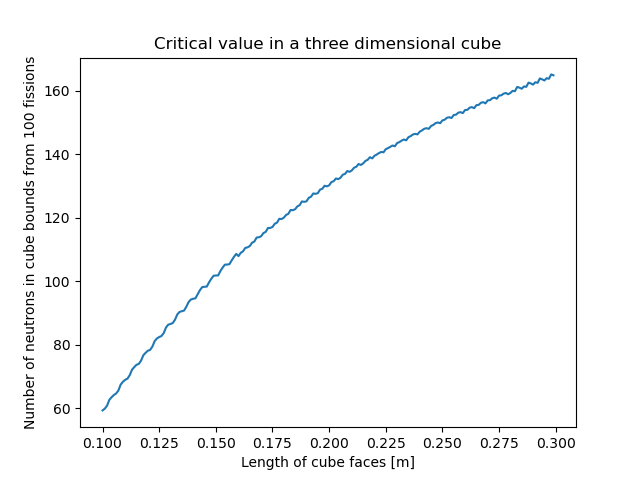
\includegraphics[width=\textwidth]{./4.png}
    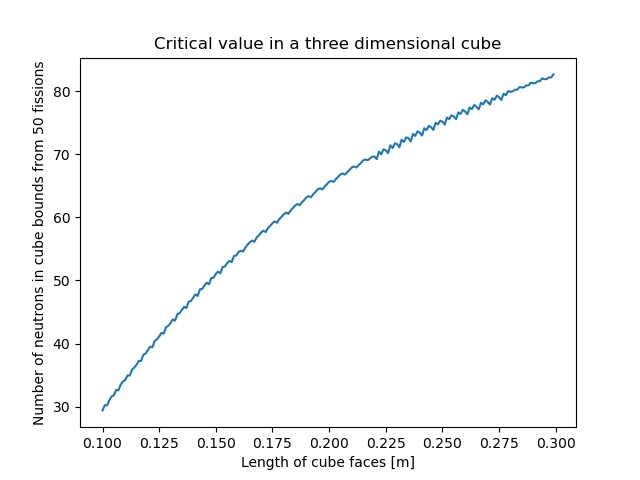
\includegraphics[width=\textwidth]{./4_2.png}
    \end{center}
    From the above graphs we can see that the critical mass does not change with a change in initial fissions $\rightarrow$ this is obviously expected from a physical standpoint and it is good that the code reflects this.
\end{document}
